\section{Results}
\label{sec:results}

After converting speech from the source speaker to target speaker, we evaluated our resort as a measure of relative distortion, according to the equation below \cite{mashimo2001evaluation}.

\begin{align*}
    MelCD = \frac{10}{\ln10}\sqrt{2\sum^{25}_{i=1}(mc_i^{conv} - mc_i^{tar})^2}
\end{align*}

Essentially, this equation gives the dB scale of distortion between two Mel Cepstrums. First, we calculate the original distortion between the target and source for the same phrase. Then we calculate the difference between the converted voice and the target for VQ and Full Conversion, as shown in Figure \ref{fig:melcd} below. The results show that the \textit{MelCD}, a measure of distortion, of Full Conversion is 37.66,  and \textit{MelCD} of VQ Conversion is 39.53. The Full Conversion reduced  \textit{MelCD} by 4.77 dB compared to the original distortion between source and target, which is significant. The following two images are Figure \ref{fig:vqresult} and Figure \ref{fig:fullresult}, which display the envelope of the source, target, and converted speech for VQ and Full Conversion, respectively.

\begin{figure}[htb]
  \centering
  \centerline{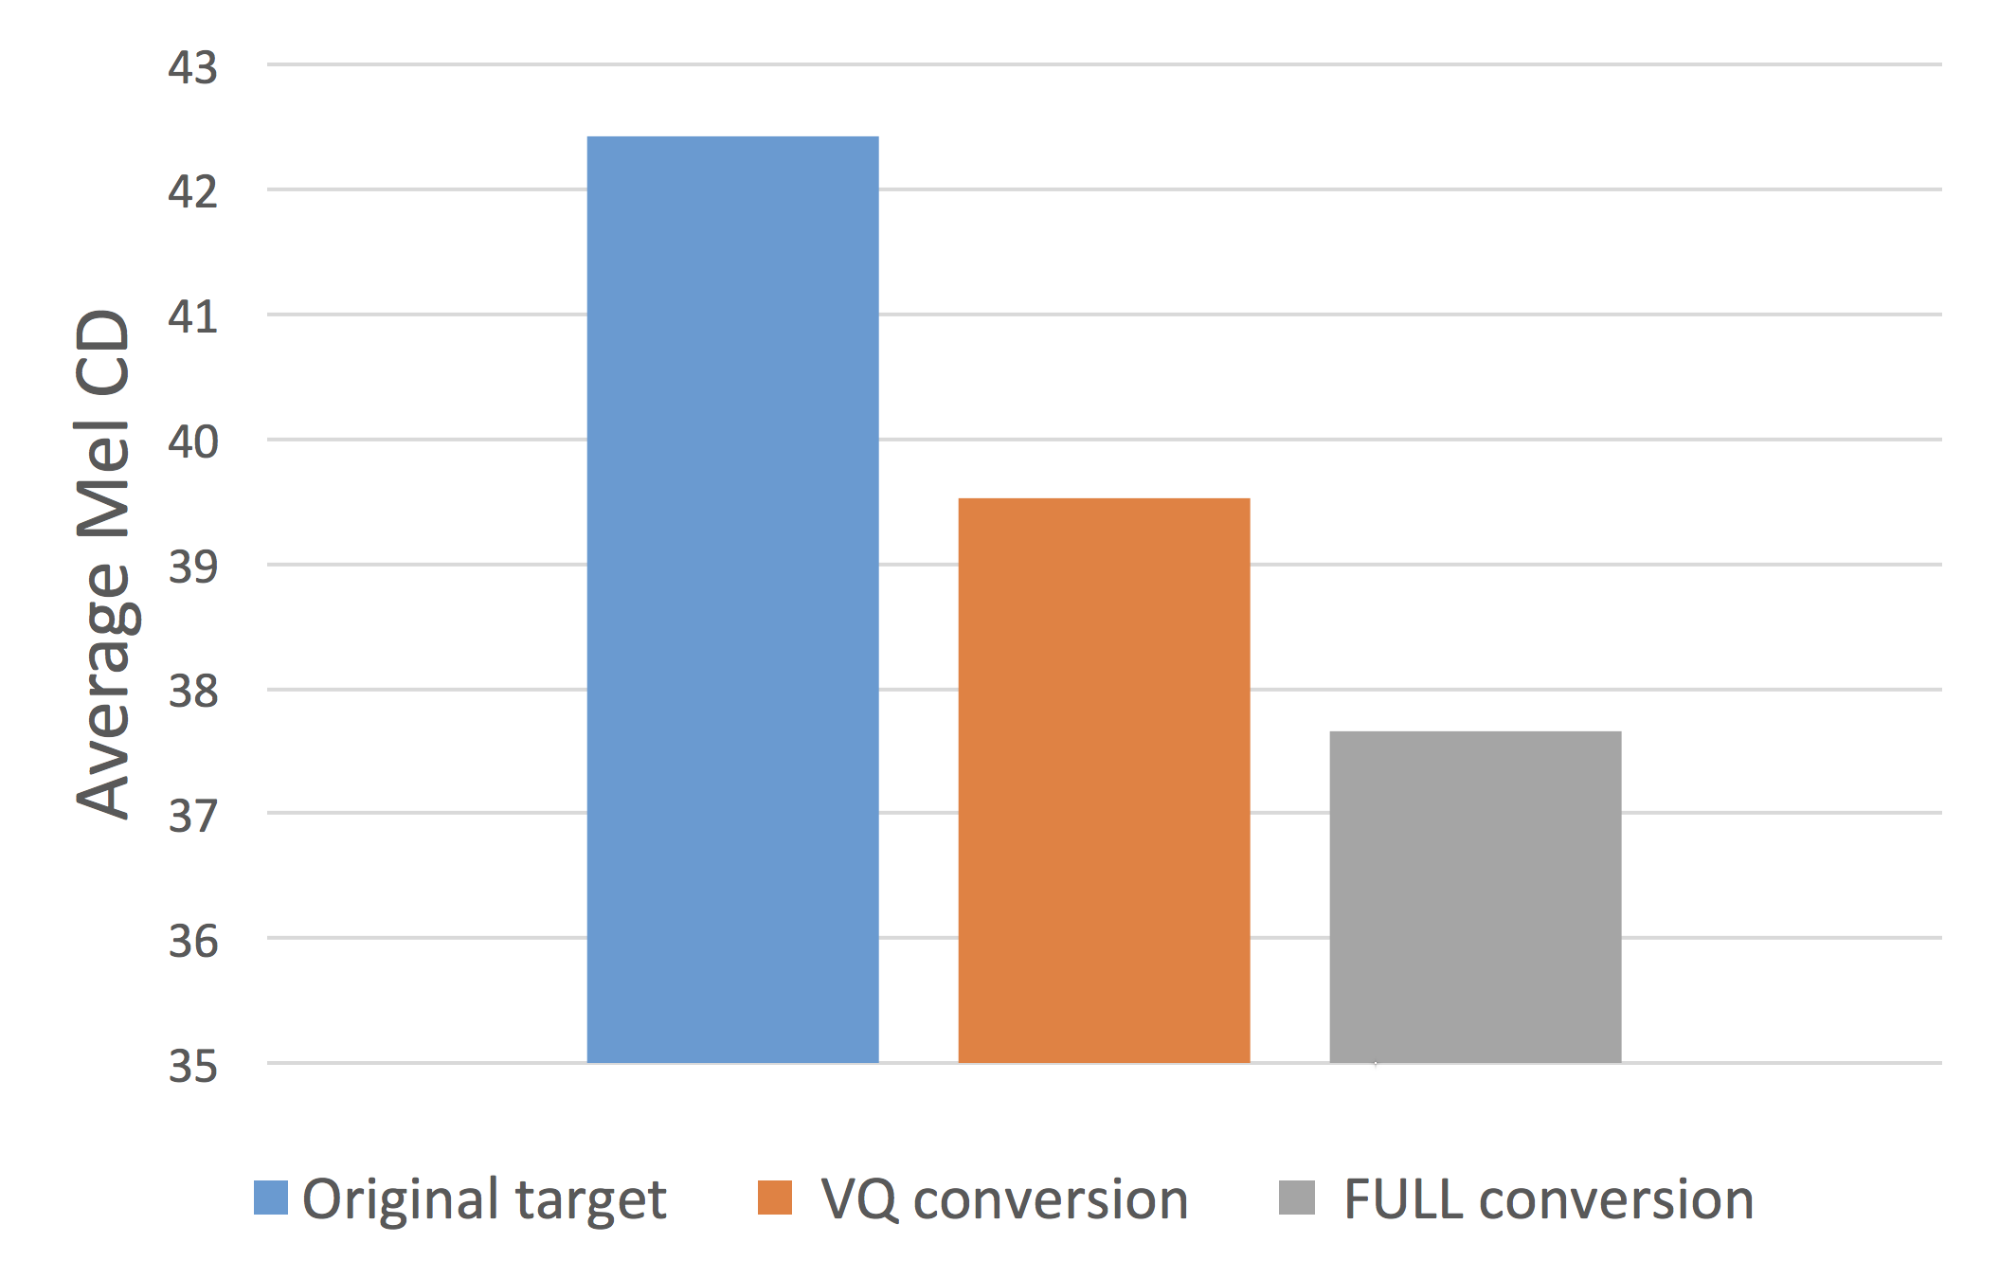
\includegraphics[width=8.5cm]{image2}}
%  \vspace{2.0cm}
\caption{The MelCD comparison of no conversion, full conversion and VQ conversion}
\label{fig:melcd}
%
\end{figure}

\begin{figure}[htb]
\begin{minipage}[b]{1\linewidth}
  \centering
  \centerline{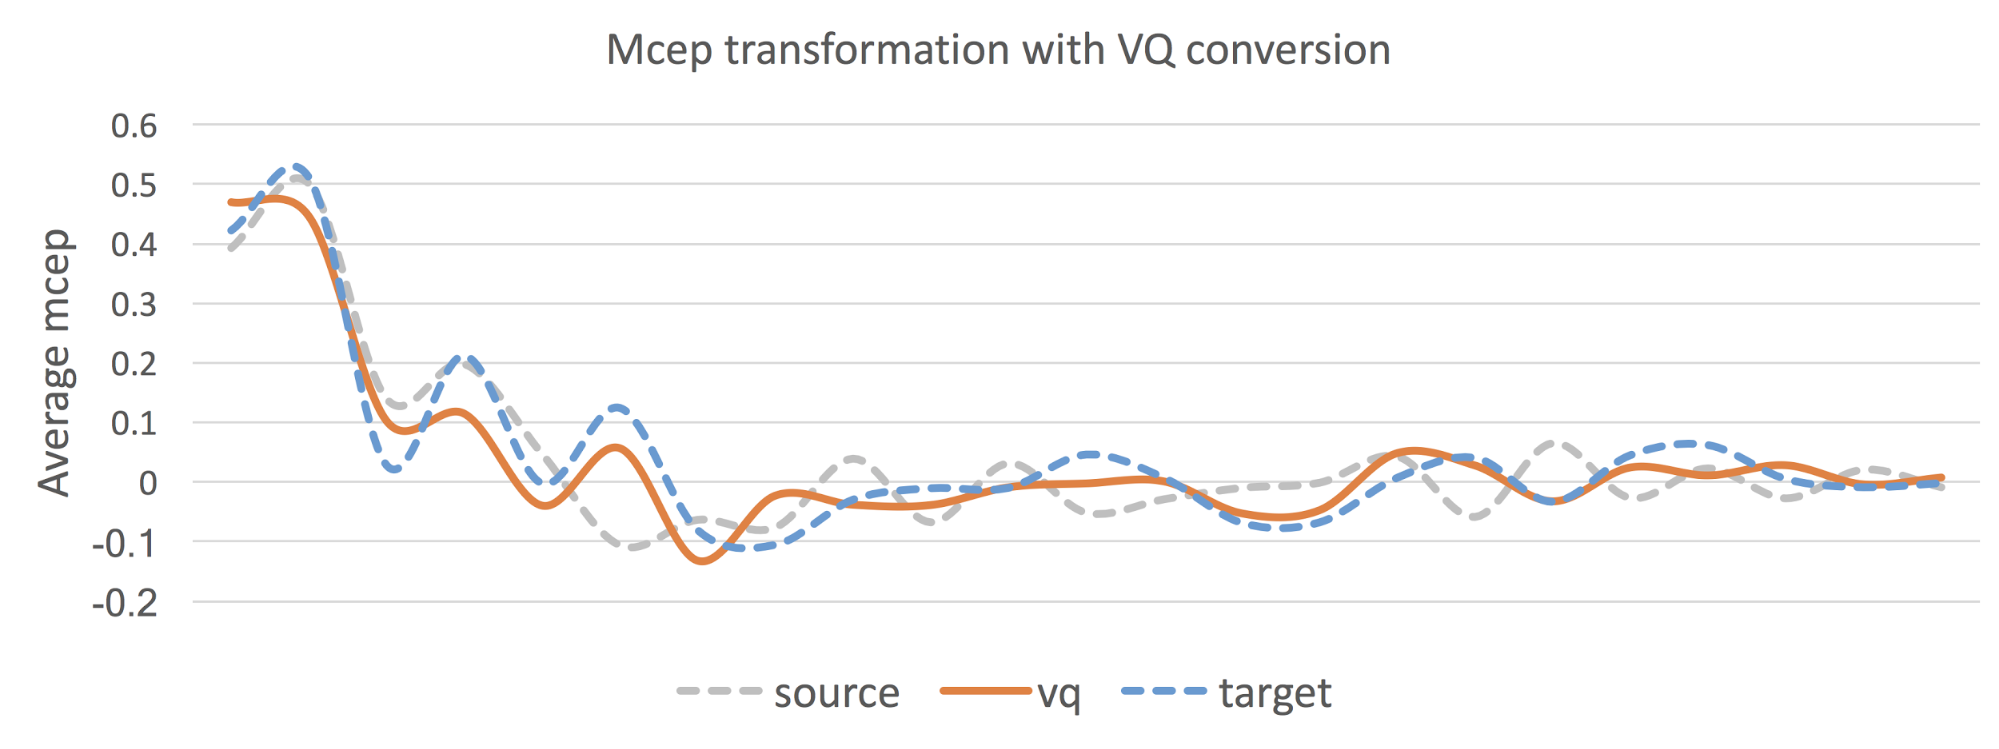
\includegraphics[width=8.5cm]{image4}}
%  \vspace{2.0cm}
\end{minipage}
\caption{Average mcep values for VQ conversion.}
\label{fig:vqresult}
\end{figure}

\begin{figure}[htb]
\begin{minipage}[b]{1\linewidth}
  \centering
  \centerline{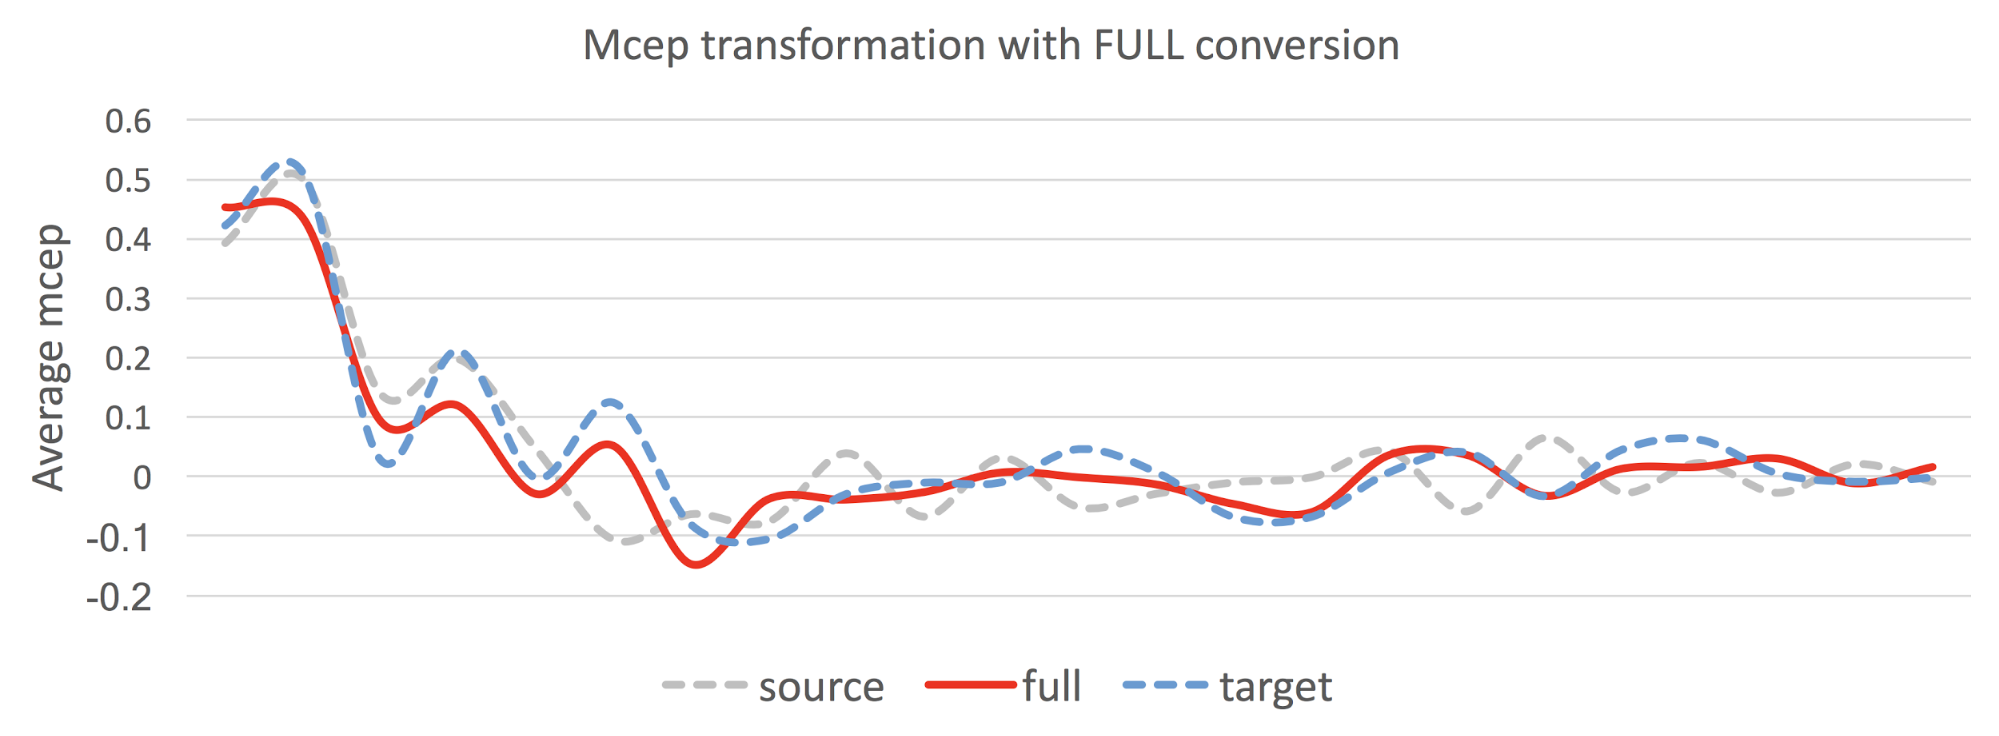
\includegraphics[width=8.5cm]{image5}}
%  \vspace{1.5cm}
\end{minipage}

\caption{Average mcep values for Full conversion.}
\label{fig:fullresult}
%
\end{figure}